\chapter{Experimental Setup}
\label{ch:ExperimentalSetup}

\section{Sensors}
\subsection{\glsentrytext{imu}}
\begin{figure}[htb]
	\centering
	\begin{subfigure}[b]{0.4\textwidth}
		\centering
		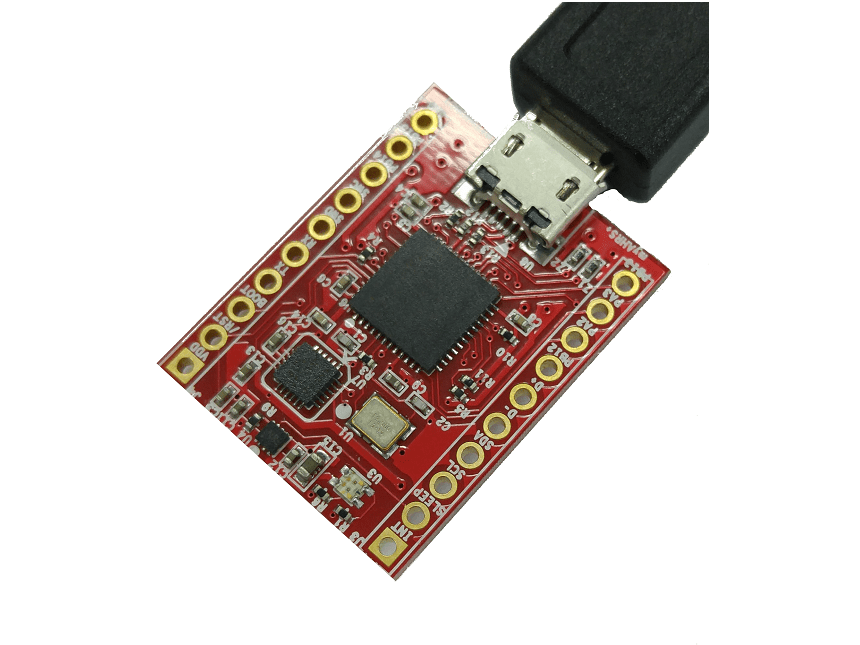
\includegraphics[width=\textwidth]{myAHRS.png}
		\caption{Withrobot myAHRS+ \cite{Withrobot2017}}
		\label{fig:imu_myahrs}
	\end{subfigure}
	% \hfill
	\begin{subfigure}[b]{0.4\textwidth}
		\centering
		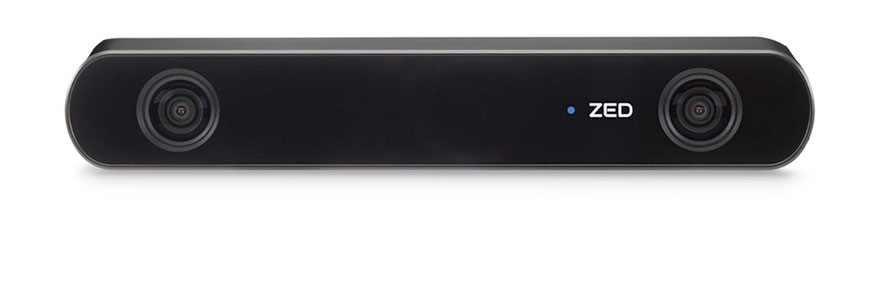
\includegraphics[width=\textwidth]{zed2i.jpg}
		\caption{Stereolabs ZED 2i camera with integrated \acrshort{imu} \cite{Stereolabs2019}}
		\label{fig:imu_zed}
	\end{subfigure}
	\caption{The two used \acrshort{imu}s}
	\label{fig:imus_used}
\end{figure}
Two different \gls{imu}s will be used for the experiment.
The first one being the Withrobot myAHRS+, a low-cost high performance \gls{ahrs}.
An \gls{ahrs} contains an \gls{imu} and outputs the raw measurements, but also has an on-board processing system which estimates attitude and heading.
The myAHRS+ uses an extended Kalman filter for the estimation and outputs the estimation in quaternion form and also in Euler angles.
The second \gls{imu} used during the experiment is integrated in the Stereolabs ZED 2i stereo camera.
The ZED 2i camera has two horizontally displaced lenses, allowing for stereo vision and thus also depth estimation.
A barometer, temperature sensor and an \gls{imu} are integrated as well.
The ZED 2i is also an \gls{ahrs} and estimates the orientation using \todo{what kind of filter?}.
Both sensors are connected to the computer via USB.
The specifications of each \gls{imu} can be read in \cref{tab:imu_datasheets}.
Because no information about the noise density or random walk of the myAHRS+ \gls{imu} could be found, a manual estimation of the error was done using the package \texttt{allan\_variance\_ros}~\footnote{\url{https://github.com/gaowenliang/imu_utils}}.
It analyzes the Allan variance from \gls{imu} measurement data recorded over a two-hour period, during which the \gls{imu} has not been moved.
\iquest{How to cite/link to a GitHub package?}

\begin{table}[ht]
	\centering
	\caption{Comparison of the two used \gls{imu}s \cite{Withrobot2017, Stereolabs2019}}
	\label{tab:imu_datasheets}
	\begin{tabular}[t]{lcc}
		\toprule
		                            & \textbf{myAHRS+}                                                      & \textbf{ZED 2i \gls{imu}}                                             \\
		\midrule
		Accelerometer range         & $\pm\SI{16}{\g}$                                                      & $\pm\SI{8}{\g}$                                                       \\
		Gyroscope range             & $\pm\SI{2000}{\degree\per\second}$                                    & $\pm\SI{1000}{\degree\per\second}$                                    \\
		Magnetometer range          & $\pm\SI{1200}{\micro\tesla}$                                          & $\pm\SI{2500}{\micro\tesla}$                                          \\
		Rate                        & \SI{100}{\hertz}                                                      & \SI{400}{\hertz}                                                      \\
		Accelerometer noise density & \SI{4.502e-3}{\frac{\metre}{\second\squared}\frac{1}{\sqrt{\hertz}}}  & \SI{1.148e-3}{\frac{\metre}{\second\squared}\frac{1}{\sqrt{\hertz}}}  \\
		Accelerometer random walk   & \SI{7.337e-5}{\frac{\metre}{\second\cubed}\frac{1}{\sqrt{\hertz}}}    & \SI{6.458e-5}{\frac{\metre}{\second\cubed}\frac{1}{\sqrt{\hertz}}}    \\
		Gyroscope noise density     & \SI{1.674e-4}{\frac{\radian}{\second}\frac{1}{\sqrt{\hertz}}}         & \SI{8.254e-5}{\frac{\radian}{\second}\frac{1}{\sqrt{\hertz}}}         \\
		Gyroscope random walk       & \SI{5.042e-6}{\frac{\radian}{\second\squared}\frac{1}{\sqrt{\hertz}}} & \SI{1.632e-7}{\frac{\radian}{\second\squared}\frac{1}{\sqrt{\hertz}}} \\
		\bottomrule
	\end{tabular}
\end{table}


\subsection{\glsentrytext{lidar}}
Two different \gls{lidar}s will be used during the experiment.
The RS-Bpearl and the Velodyne UltraPuck, see \cref{fig:lidars_used}.
The most relevant specifications of the two \gls{lidar}s can be seen in \cref{tab:lidar_datasheets}.
Both are mechanical \gls{lidar}s and have the same number of laser channels, but the Velodyne has a significant better vertical resolution, due to the smaller vertical \gls{fov}.
Both \gls{lidar}s need an external power supply and transfer the data over Ethernet.
\begin{table}[ht]
	\centering
	% todo: Manual citation prop wrong
	\caption{Comparison of the two used \acrshort{lidar}s \cite{RoboSense2020, Velodyne2018}}
	\label{tab:lidar_datasheets}
	\begin{tabular}[t]{lcc}
		\toprule
		                      & \textbf{RS-Bpearl}          & \textbf{Velodyne Ultra Puck}                  \\
		\midrule
		Channels              & 32                          & 32                                            \\
		Range                 & \SI{100}{\metre}            & \SI{200}{\metre}                              \\
		Range accuracy        & $\pm\SI{3}{\centi\metre}$   & $\pm\SI{3}{\centi\metre}$                     \\
		Horizontal \gls{fov}  & \SI{360}{\degree}           & \SI{360}{\degree}                             \\
		Vertical \gls{fov}    & \SI{90}{\degree}            & \SI{40}{\degree} (\SIrange{-25}{15}{\degree}) \\
		Horizontal resolution & \SIrange{0.2}{0.4}{\degree} & \SIrange{0.1}{0.4}{\degree}                   \\
		Vertical resolution   & \SI{2.81}{\degree}          & \SI{0.33}{\degree}                            \\
		Frame rate            & \SIrange{10}{20}{\hertz}    & \SIrange{5}{20}{\hertz}                       \\
		Laser wavelength      & \SI{905}{\nano\metre}       & \SI{903}{\nano\metre}                         \\
		% \midrule
		Points per second     & 576,000                     & 600,000                                       \\
		\bottomrule
	\end{tabular}
\end{table}%
\begin{figure}[htb]
	\centering
	\begin{subfigure}{0.3\textwidth}
		\centering
		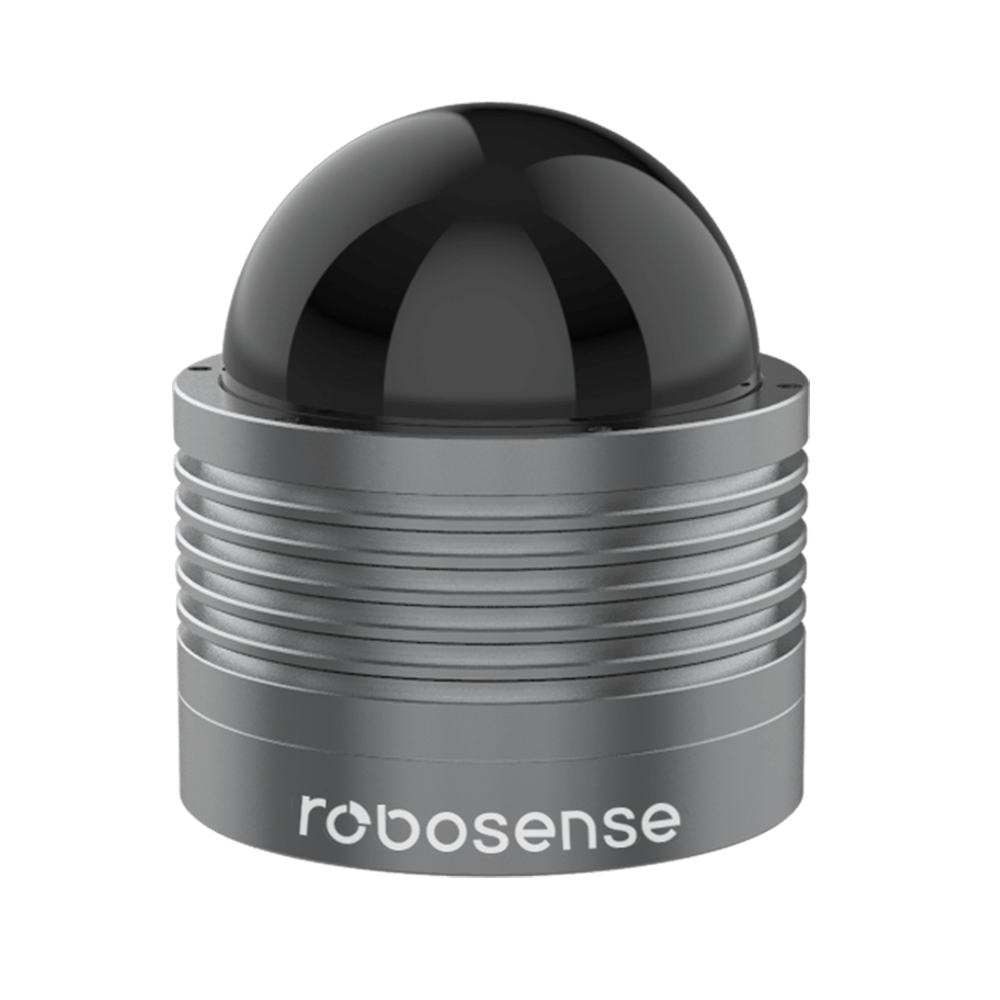
\includegraphics[width=\textwidth]{Robosense.png}
		\caption{Robosense RS-Bpearl \cite{RoboSense2020}}
		\label{fig:lidar_robosense}
	\end{subfigure}
	% \hfill
	\begin{subfigure}{0.3\textwidth}
		\centering
		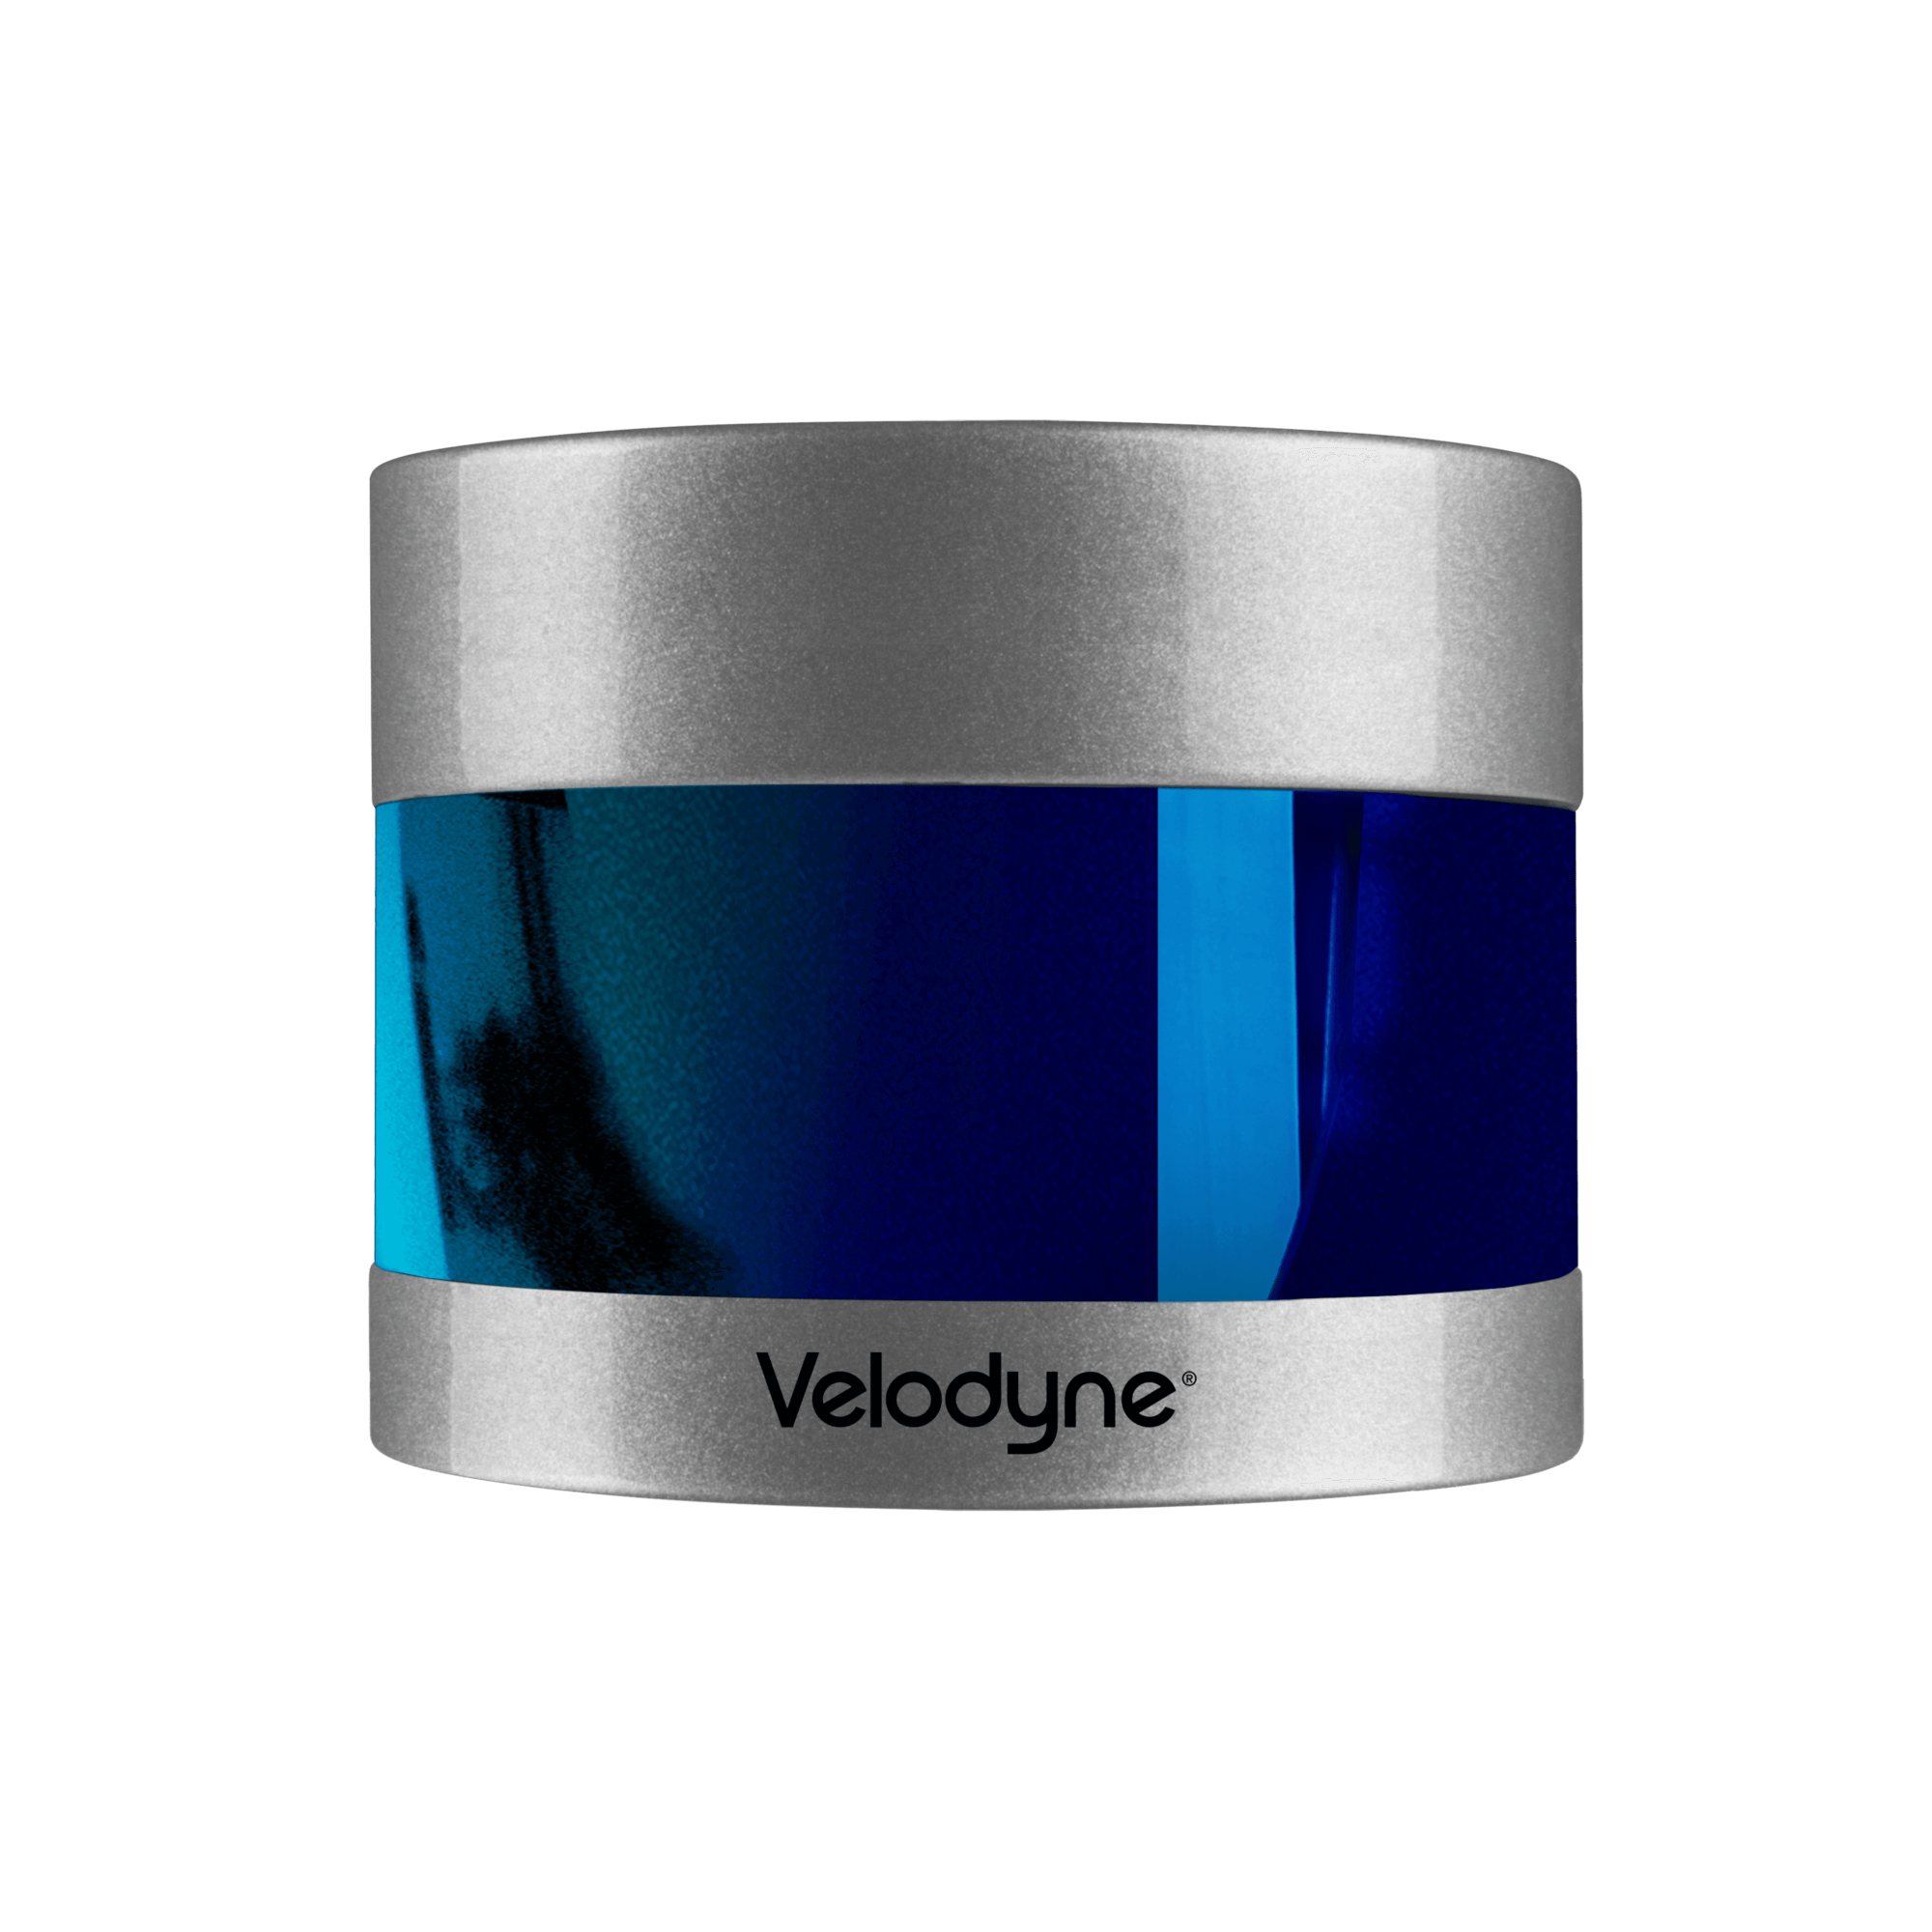
\includegraphics[width=\textwidth]{Velodyne.png}
		\caption{Velodyne Ultra puck \cite{Velodyne2018}}
		\label{fig:lidar_velodyne}
	\end{subfigure}
	\caption{The two used \gls{lidar}s}
	\label{fig:lidars_used}
\end{figure}



\section{Sensor placement}
The \gls{imu} must be placed on a rigid point of the car, such that the \gls{imu}'s position always stays the same relative to the car.
Other than that it should also be placed in the transversal center? to guarantee that the centripetal acceleration is not skewed towards one side.
The ZED 2i camera with the integrated \gls{imu} was placed on the roof of the car, because the camera images were used as well.
The myAHRS+ \gls{imu} was mounted on the floor of the car trunk.\\
\begin{figure}[htpb]
	\centering
	\documentclass[12pt]{standalone}
\usepackage{tikz}
\usepackage{tikz-dimline}		% Dimension (measure) lines for TikZ
\usetikzlibrary{angles, calc, decorations.pathmorphing, quotes, spy}

\begin{document}
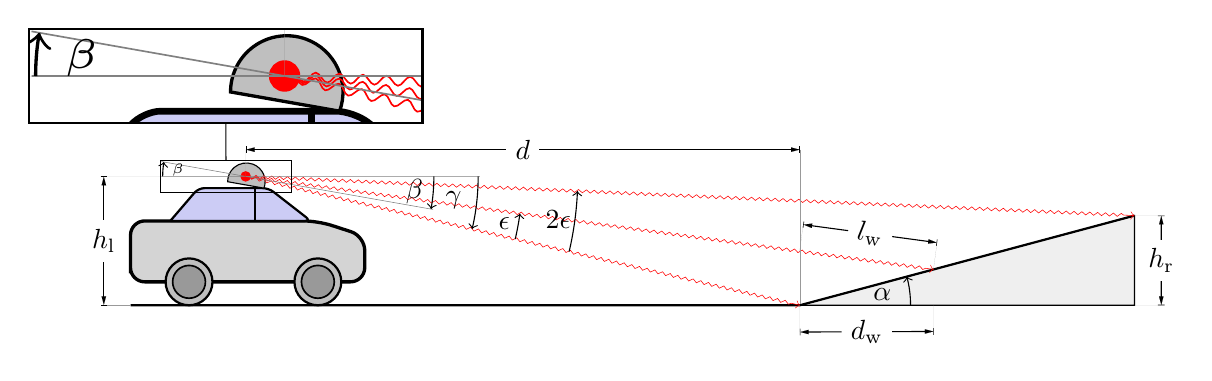
\begin{tikzpicture}[scale=0.85, spy using outlines={black, rectangle, magnification=3, width=5cm, height=1.2cm, connect spies}]
        % Define/Calc ramp parameters
        % Ramp length
        \def\rl{5};
        % Ramp angle [deg]
        \def\ra{15};
        % Ramp height
        \def\rh{{tan(\ra)*\rl}};
        % Distance of measurement line
        \def\dd{.4cm}

        % RAMP
        % Define the points
        % Left point
        \coordinate (A) at (0,0);
        % Lower right point
        \coordinate (B) at ($(A) + (\rl,0)$);
        % Upper right point
        \coordinate (C) at ($(B) + (0,\rh)$);

        % Draw and fill ramp
        \filldraw[draw=black, fill=lightgray!25] (A) -- (B) -- (C) -- cycle;
        % Draw ramp angle
        \path (A) -- (B)
        pic[draw, ->, angle radius=40pt,
                        angle eccentricity=0.75, "$\alpha$"]{angle=B--A--C};

        % Most left point at ground level
        \coordinate (D) at ($(A) + (-10,0)$);
        % Ground line
        \draw [thick] (D) -- (A) -- (C);


        % CAR
        \begin{scope}[scale=0.7]
                % Car height
                \def\ch{2}
                % Car length
                \def\cl{5}
                % Car body height
                \def\bh{\ch*0.65}
                % Roof length
                \def\rl{\cl*0.6}
                % Roof height
                \def\rh{\ch*0.35}
                % Anchor point of car body (lower left)
                \coordinate (b) at ($(D) + (0,0.5)$);
                % Offset to roof and wheels
                \coordinate (r) at ($(b) +(\cl*0.17,\ch*0.65)$);
                \coordinate (w) at ($(b) + (\cl*0.25,0)$);

                % Body
                \draw[black, fill=black!17, rounded corners=1.2ex, very thick]
                (b) -- ++(0,\bh) -- ++(\cl*1/5,0) --  ++(\cl*3/5,0) -- ++(\cl*1/5,-\bh*0.25)
                -- ++(0, -\bh*0.75) -- (b) -- cycle;
                % Roof
                \draw[very thick, rounded corners=0.5ex, fill=black!20!blue!20!white,thick]
                (r) -- ++(0.2*\rl,\rh) -- ++(0.5*\rl,0) -- ++(0.3*\rl,-\rh) -- (r);
                \draw[thick] (r)++(\rl*0.6,0) -- ++(0,\rh);

                % Wheels
                \draw[draw=black,fill=gray!50,thick] (w) circle (.5);
                \draw[draw=black,fill=gray!50,thick] (w) ++(\cl*0.55,0) circle (.5);
                % Inner wheels
                \draw[draw=black,fill=gray!80,semithick] (w) circle (.35);
                \draw[draw=black,fill=gray!80,semithick] (w) ++(\cl*0.55,0) circle (.35);

                % Lidar
                % Lidar pitch angle
                \def\lpa{10};
                \draw[black, fill=gray!50] ($(r) + (\cl*0.40,\rh)$) coordinate (le) arc(-\lpa*2:180:0.4) --cycle;

                % Car middle point
                \coordinate (m) at (\cl*0.5, \bh*0.5);
                % Lidar middle point
                \coordinate (lm) at ($(le) + (-0.39,0.25)$);
                \filldraw[red] (lm) circle(.1);
                \coordinate (idk) at ($(A)!0.4!(C)$);

                % Laser lines
                \draw[->,color=red,very thin,decorate,decoration={snake,amplitude=.2mm,segment length=1mm,post length=1mm}] (lm) -- (A)
                pic[draw, black, ->, thin, angle radius=100pt, angle eccentricity=0.95,
                                "$\epsilon$"]{angle=A--lm--idk};
                \draw[->,color=red,very thin,decorate,decoration={snake,amplitude=.2mm,segment length=1mm,post length=1mm}] (lm) -- ($(A)!0.4!(C)$);
                \draw[->,color=red,very thin,decorate,decoration={snake,amplitude=.2mm,segment length=1mm,post length=1mm}] (lm) -- ($(A)!1!(C)$)
                pic[draw, black, ->, thin, angle radius=120pt, angle eccentricity=0.95,
                                "$2\epsilon$"]{angle=A--lm--C};


                % lidar mount angle
                % Length of angle helper line
                \def\hl{4};
                \def\hll{1.8};
                \coordinate (bleb) at ($(lm) + (\hl+1, 0)$);
                \coordinate (blab) at ($(lm) + (\hl, -{tan{\lpa}*\hl})$);
                \coordinate (blub) at ($(lm) + (-\hll, 0)$);
                \coordinate (blob) at ($(lm) + (-\hll, +{tan{\lpa}*\hll})$);
                \draw[draw=gray, very thin] (blub) -- (lm) -- (blob)
                pic[draw, black, thin, <-, angle radius=30pt,
                                angle eccentricity=0.82, "\tiny $\beta$"]{angle=blob--lm--blub};
                \draw[draw=gray, very thin] (bleb) -- (lm) -- (blab)
                pic[draw, black, thin, <-, angle radius=68pt,
                                angle eccentricity=0.9, "$\beta$"]{angle=blab--lm--bleb};
                \path (bleb) -- (lm) -- (A)
                pic[draw, <-, thin, angle radius=84pt,
                                angle eccentricity=0.9, "$\gamma$"]{angle=A--lm--bleb};

        \end{scope}

        % \filldraw[green] (idk) circle(.2);
        \dimline[extension start length=\dd, extension end length=\dd+1.9cm] {($(lm)+(0,\dd)$)}{($(lm -| A)+(0,\dd)$)}{$d$};
        % \dimline[extension start length=-\dd, extension end length=-\dd] {($(A)+(0,-\dd)$)}{($(B)+(0,-\dd)$)}{$l_\mathrm{r} $};
        \dimline[extension start length=-\dd, extension end length=-\dd, label style={sloped=false}] {($(B)+(\dd,0)$)}{($(C)+(\dd,0)$)}{$h_\mathrm{r}$};
        \dimline[extension start length=\dd, extension end length=\dd+1.7cm, label style={sloped=false}] {($(D)+(-\dd,0)$)}{($(lm -| D)+(-\dd,0)$)}{$h_\mathrm{l} $};

        % \dimline[extension start length=\dd, extension end length=-\dd] {($(idk)+(\dd,0)$)}{($(idk)+(\dd,-0.53)$)}{};
        % \dimline[extension start length=0, extension end length=0, label style={right, fill=none, sloped=false}] {(idk)}{($(idk)+(0,-0.53)$)}{$h_\mathrm{w}$};
        \dimline[extension start length=-\dd, extension end length=-\dd] {($(A)+(0,-\dd)$)}{($(idk)+(0,-\dd-15)$)}{$d_\mathrm{w} $};
        \dimline[extension start length=\dd, extension end length=\dd] {($(A)+(0.05,-\dd+\dd+34.3)$)}{($(idk)+(0.05,\dd)$)}{$l_\mathrm{w} $};

        % \spy[black] on ($(lm) + (-0.42, 0)$) in node at (3,4);
        \spy on ($(lm) + (-0.25, 0)$) in node at ($(lm) + (-0.3, 1.5)$);

\end{tikzpicture}
\end{document}
	\caption{Mounting of the \acrshort{lidar}. Variable description in \cref{tab:lidar_mount}}
	\label{fig:tikz_lidar_mount}
\end{figure}
\begin{table}[htbp]
	\centering
	\caption{Some params}
	\label{tab:lidar_mount}
	\begin{tabular}[t]{clc}
		\toprule
		\textbf{Variable} & \textbf{Description}                                   & \textbf{Unit} \\
		\midrule
		$h_\mathrm{l} $   & \gls{lidar} height above ground                        & \si{\metre}   \\
		$d$               & Distance to ramp                                       & \si{\metre}   \\
		$h_\mathrm{r}$    & Height of ramp                                         & \si{\metre}   \\
		$l_\mathrm{w}$    & Light travel distance from ramp start to contact point & \si{\metre}   \\
		$d_\mathrm{w}$    & Distance from ramp start to contact point              & \si{\metre}   \\
		$\alpha$          & Ramp angle                                             & \si{\degree}  \\
		$\beta$           & \gls{lidar} mount angle                                & \si{\degree}  \\
		$\gamma$          & True angle?!                                           & \si{\degree}  \\
		$\epsilon$        & \gls{lidar} vertical resolution                        & \si{\degree}  \\
		$n$               & Number of laser channels                               &               \\
		\bottomrule
	\end{tabular}
\end{table}
The \gls{lidar} will be placed on top of the car, to get a greater \gls{fov}.
The pitch angle $\beta$ at which the \gls{lidar} will be mounted should be chosen such that the number of points in the area at the beginning of the ramp are maximized.
This allows for the most accurate distinction between planes of different inclination angles and therefore also a good distance estimation.
Because the distance to the ramp is not constant due to the movement of the car, the optimization can only be done for a specific distance.
The coordinates at which the lasers hit the ground and ramp depend on the height of the \gls{lidar} $h_\mathrm{l}$, the distance to the ramp $d$, the angle of the ramp $\alpha$, the angle $\beta$ at which the \gls{lidar} has been mounted on the car and finally on the vertical resolution $\epsilon$ and \gls{fov} of the \gls{lidar}.
The coordinates can be calculated in the following way.\\
The angle $\gamma$ between the plane parallel to the ground at \gls{lidar} height and each laser wave is defined as
\begin{equation}
	\gamma = \beta - i\epsilon
\end{equation}
with $i \in [0,1,2,\dots,n]$ being the "laserID" starting from the lowest opening angle and going to the highest and $n$ being the number of laser channels.
On flat ground the distance at which the laser waves hit the ground can be calculated by
\begin{equation}
	x = \tan(\ang{90} - \gamma) h_\mathrm{l}.
	\label{eq:ground_points}
\end{equation}
With a ramp, the assumption from \cref{eq:ground_points} does not hold anymore.
The light does not travel as far.
The height above ground, when the light is at the beginning of the ramp can be calculated by
\begin{equation}
	h_\mathrm{w,start} = h_\mathrm{l} - d\tan(\gamma)
\end{equation}
The distance $l_\mathrm{w}$ which the light travels from the beginning of the ramp to the contact point with the ramp can be calculated using the law of sines
\begin{align}
	l_\mathrm{w} & = \frac{h_\mathrm{w,start} }{\sin(\alpha + \gamma)} \sin(\ang{90} - \alpha) \\
	             & = -\frac{h_\mathrm{w,start} }{\sin(\alpha + \gamma)} \cos(\alpha)
\end{align}
The travelled distance along the x-axis from the start of the ramp to the contact point is then
\begin{equation}
	d_\mathrm{w}  = l_\mathrm{w} \sin(\ang{90} - 2\alpha - \gamma)
\end{equation}
which results in the total x distance from the \gls{lidar}
\begin{equation}
	d_\mathrm{hit} = d + d_\mathrm{w}
\end{equation}
or in full length
\begin{equation}
	\label{eq:final_equation}
	d_\mathrm{hit} = d + \frac{h_\mathrm{l} - d\tan(\gamma)}{\sin(\alpha + \gamma)} \cos(-\alpha) \sin(\ang{90} - 2\alpha - \gamma)
\end{equation}
Using \cref{eq:final_equation} and optimizing $\beta$ such that the number of points in the area at the start of the ramp are maximized, the optimal mounting pitch angle $\beta$ for the two \gls{lidar}s has been found with $\beta_\mathrm{velodyne} = \ang{0}$ and $\beta_\mathrm{robos} = \ang{20}$.
The optimization was done for a distance of \SI{10}{\metre} to the ramp.
The angle between the two \gls{lidar}s differs due to the different starting opening angle of \SI{-25}{\degree} and \SI{0}{\degree} for the Velodyne and Robosense respectively.
\iimprov{Improve text and table param description}


\section{Car}
The car used in the experiment is an eGolf 2017.
Being an electric car it provides better vibration properties than a car with an internal combustion engine, which means that the \gls{imu} measurements are less influenced by external noise.
The car has been "hacked" which allows among other things for the reading of the wheel ticks by tapping the signals from the CAN bus.
Unfortunately the wheel speed readings are only available in this "hacked" state, in which the output power of the motor is limited.
In this mode, the maximum speed is capped at \SI{5}{\kilo\metre\per\hour} and the power is not enough to allow for the traversing of ramps.
The car can only make it about halfway up.
Because of that, the normal mode was used to drive between different levels.
Before driving down, the mode was switched again to also provide the wheel speed measurements.
The car has a PC in the booth, at which all the sensors were connected to.
\iimprov{Text is bad e.g. "hacked" }
\missingfigure{Picture of eGolf}



\section{Garage}
\missingfigure{Picture of ramps and/or figure of ramps showing angles}
\itodo{Think of a good way to measure the true angle of the ramps}
\begin{figure}
	\begin{subfigure}{.3\linewidth}
		\centering
		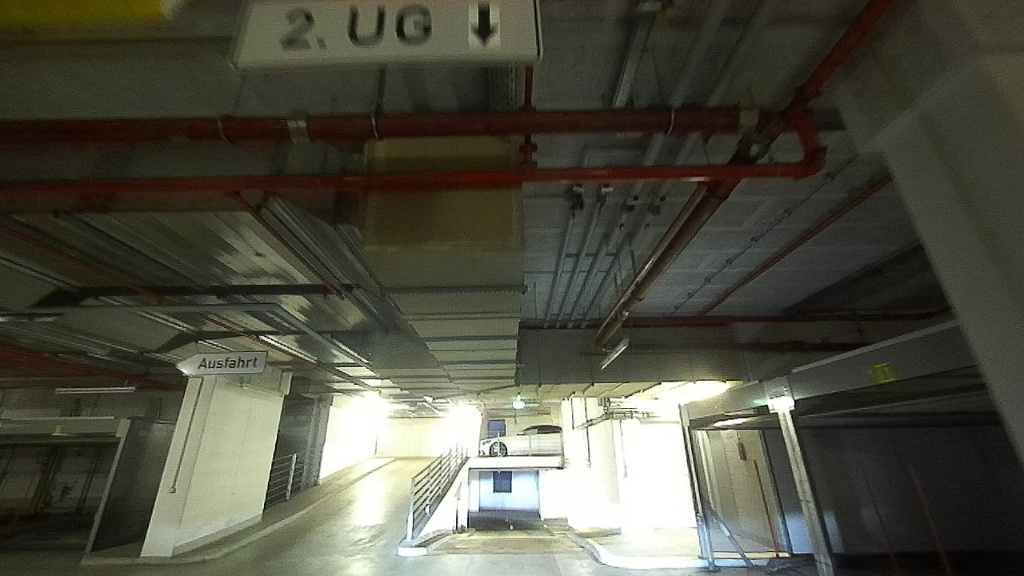
\includegraphics[width=1\linewidth]{d_d2r.jpg}
	\end{subfigure}
	\hfill
	\begin{subfigure}{.3\linewidth}
		\centering
		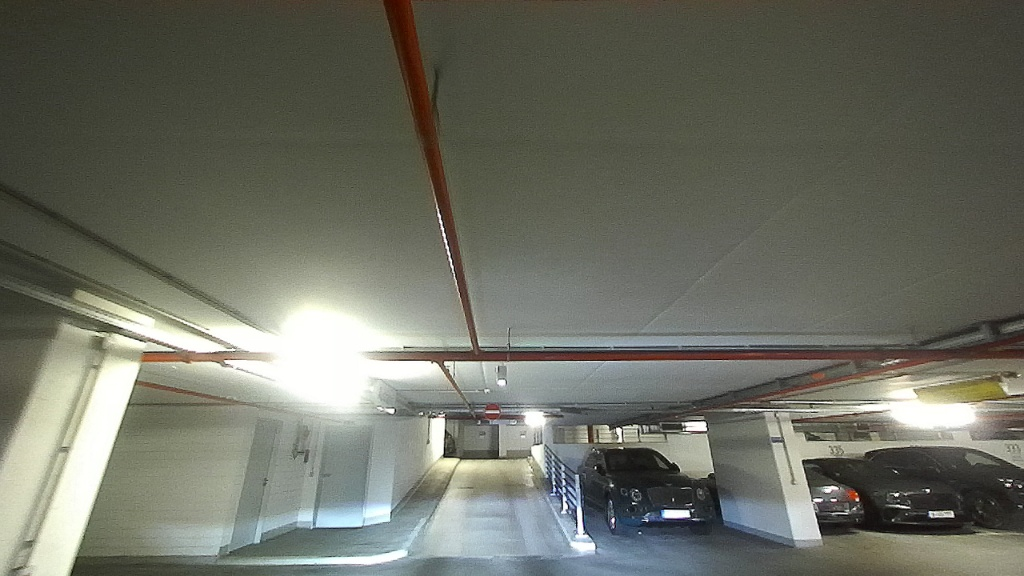
\includegraphics[width=1\linewidth]{u_c2s.jpg}
	\end{subfigure}
	\hfill
	\begin{subfigure}{.3\linewidth}
		\centering
		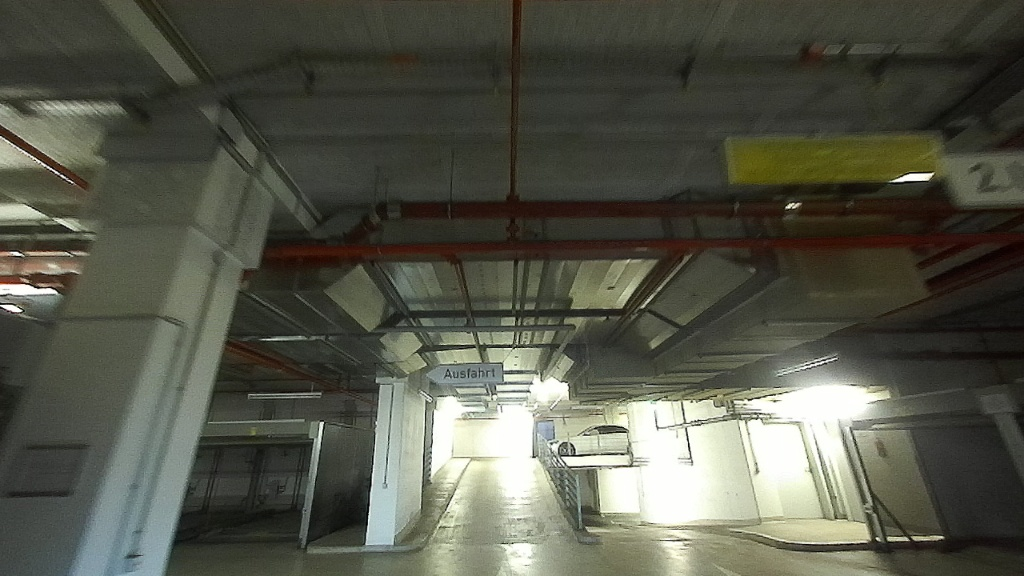
\includegraphics[width=1\linewidth]{u_d2e.jpg}
	\end{subfigure}
\end{figure}